%%===========================================================%%
%%                                                           %%
%%                        CORRECTIONS                        %%
%%                                                           %%
%%===========================================================%%


\chapter{Corrections}\label{chap:corrections}

\section{Method of corrections application}
\begin{equation}
  \frac{d\sigma}{dq} = \frac{1}{\Delta q} \times \frac{1}{\varepsilon} \times \frac{N^{\mathit{w}}-N^{\mathit{w}}_\textrm{bkgd}}{\mathit{L}_{\textrm{int}}^{\textrm{eff}}}
\end{equation}

%remembed about accounting for RP trigger eff!!!
\begin{equation}\label{eq:effectiveLumi}
	\mathit{L}_{\textrm{int}}^{\textrm{eff}} = \sum\limits_{\textrm{run}}\mathit{L}_{\textrm{int}}^{\textrm{run}} \times \epsilon_{\textrm{veto}}(L^{\textrm{run}})
\end{equation}
% \left(\epsilon_{\textrm{veto}}^{\textrm{online}} \oplus \epsilon_{\textrm{veto}}^{\textrm{offline}}(L_{\textrm{run}}) \right)

\begin{equation}
	\varepsilon = \epsilon_{\textrm{\tiny ET/IT}} \times \epsilon_{\textrm{vrtx}}(q) \times \epsilon_{\ref{enum:CutZVx}} \times \epsilon_{\ref{enum:CutDeltaZVx}} \times \epsilon_{\ref{enum:CutMissingPt}} \times \epsilon_{\textrm{\tiny PID}}(q)
\end{equation}

\begin{equation}
	N^{\mathit{w}} = \sum\limits_{\textrm{event}}\mathit{w}_{\textrm{event}}
\end{equation}



\begin{equation}
	\mathit{w} = \left[\prod\limits_{\textrm{sign}} \epsilon_{\textrm{\tiny TOF}}(\textrm{sign}, \textrm{PID}, p_{T},z_{vx},\eta)  \times \prod\limits_{\textrm{sign}} \epsilon_{\textrm{\tiny TPC}}(\textrm{sign}, \textrm{PID}, p_{T},z_{vx},\eta) \times \prod\limits_{\textrm{side}}\epsilon_{\textrm{\tiny RP}}^{\textrm{side}}(p_{x},p_{y}) \right]^{-1},
\end{equation}
\[\textrm{sign}\in\{+,-\},~~\textrm{side}\in\{E,W\}\]
% ()




\section{Efficiencies and acceptances}

In this section we present calculation of all efficiencies except TPC track reconstruction and TOF hit reconstruction and matching efficiency, which were discussed and presented in Ref.~\cite{supplementaryNote}.

\subsection{Trigger efficiency}\label{sec:triggerEff}
\subsubsection{Online veto (BBC-small and ZDC veto)}
%---------------------------
\begin{figure}[ht!]
\centering%
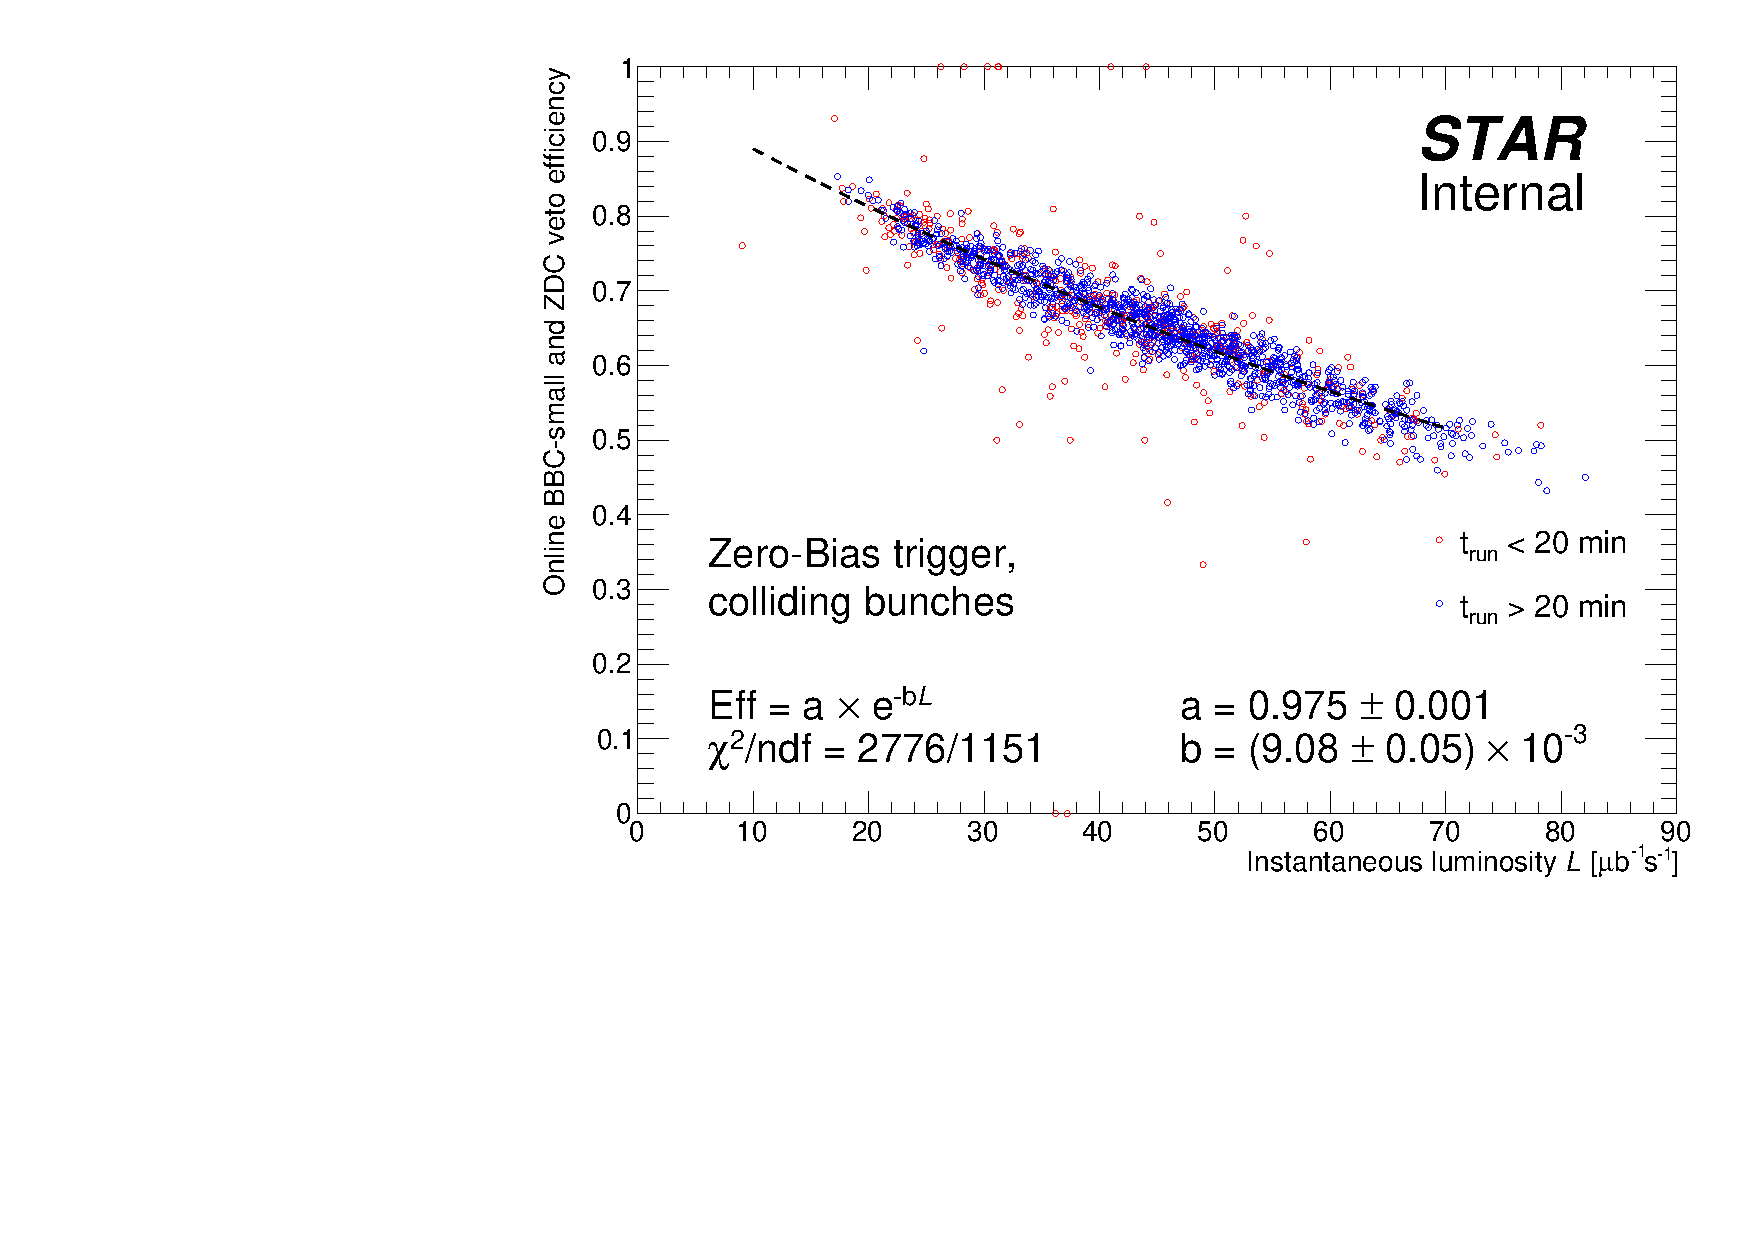
\includegraphics[width=0.65\linewidth,page=1]{graphics/corrections/OnlineVetoEffVsInstLumi_graph.pdf}%
\caption{Overall efficiency of the online BBC-small and ZDC veto as a function of instantaneous luminosity.}\label{fig:onlineVetoEff}%
\end{figure}
%---------------------------
\subsubsection{RP triggering efficiency}
\subsubsection{Up and Down RP combination veto}
\subsection{Cuts efficiency}\label{sec:cutsEff}
\subsubsection{TPC \texorpdfstring{$z$}{z}-vertex cut~(\ref{enum:CutZVx})}
\subsubsection{TPC-RP \texorpdfstring{$z$}{z}-vertex matching~(\ref{enum:CutDeltaZVx})}
\subsubsection{Primary vertices limit~(\ref{enum:CutPrimVx}), BBC-large veto~(\ref{enum:CutBbcLarge}) and TOF clusters limit~(\ref{enum:CutTofClusters})}
%---------------------------
\begin{figure}[ht!]
\centering%
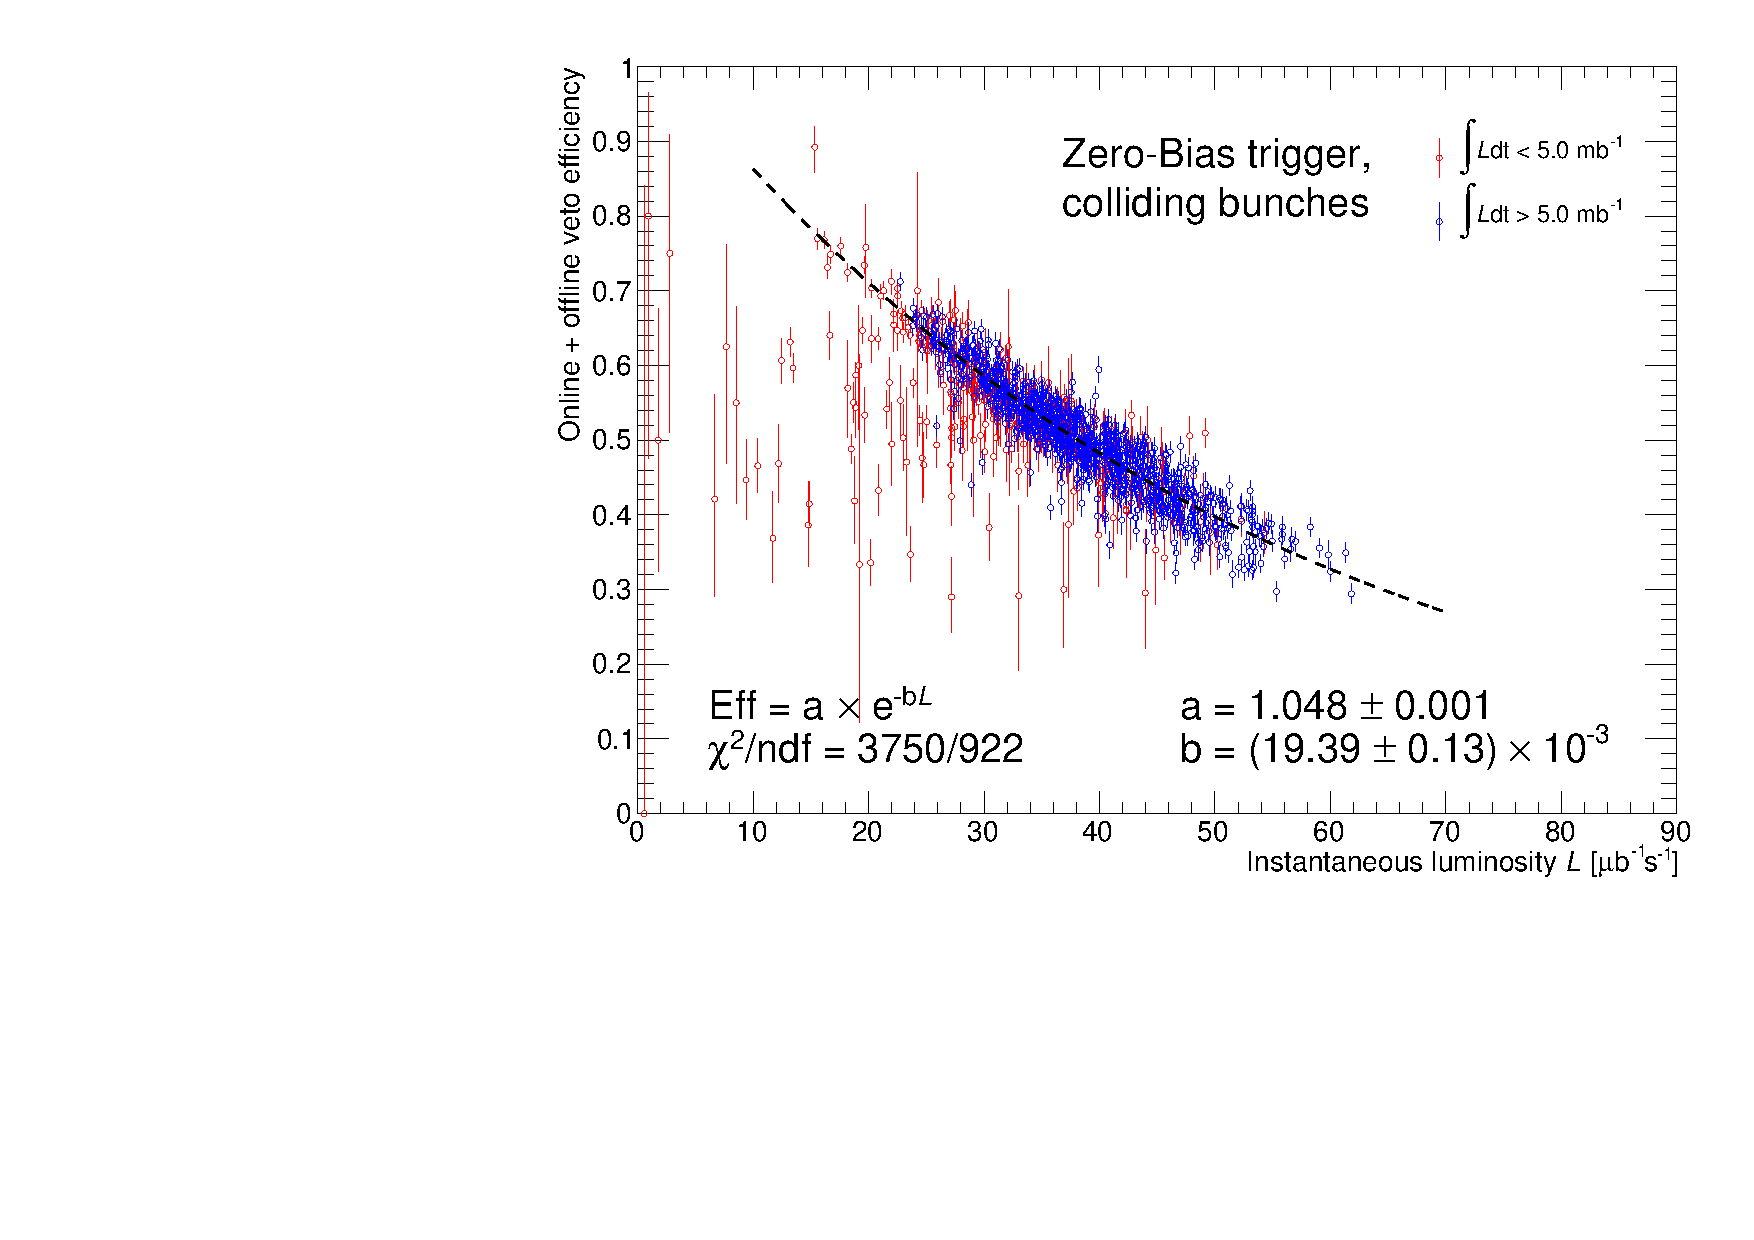
\includegraphics[width=0.65\linewidth,page=1]{graphics/corrections/OnlineAndOfflineVetoEffVsInstLumi_graph.pdf}%
\caption{Overall efficiency of the online BBC-small and ZDC veto, primary vertices limit~(\ref{enum:CutPrimVx}), BBC-large veto~(\ref{enum:CutBbcLarge}) and TOF clusters limit~(\ref{enum:CutTofClusters}) as a function of instantaneous luminosity.}\label{fig:onlineAndOfflineVetoEff}%
\end{figure}
%---------------------------
\subsubsection{Missing \texorpdfstring{$p_{T}$}{pT} cut~(\ref{enum:CutMissingPt})}
\subsubsection{Particle identification~(\ref{enum:CutPid})}


%---------------------------
\begin{figure}[ht!]
\centering
\parbox{0.315\textwidth}{
  \centering
  \begin{subfigure}[b]{\linewidth}{
                \subcaptionbox{\label{fig:sqMassTof_DataVsMC_pion}}{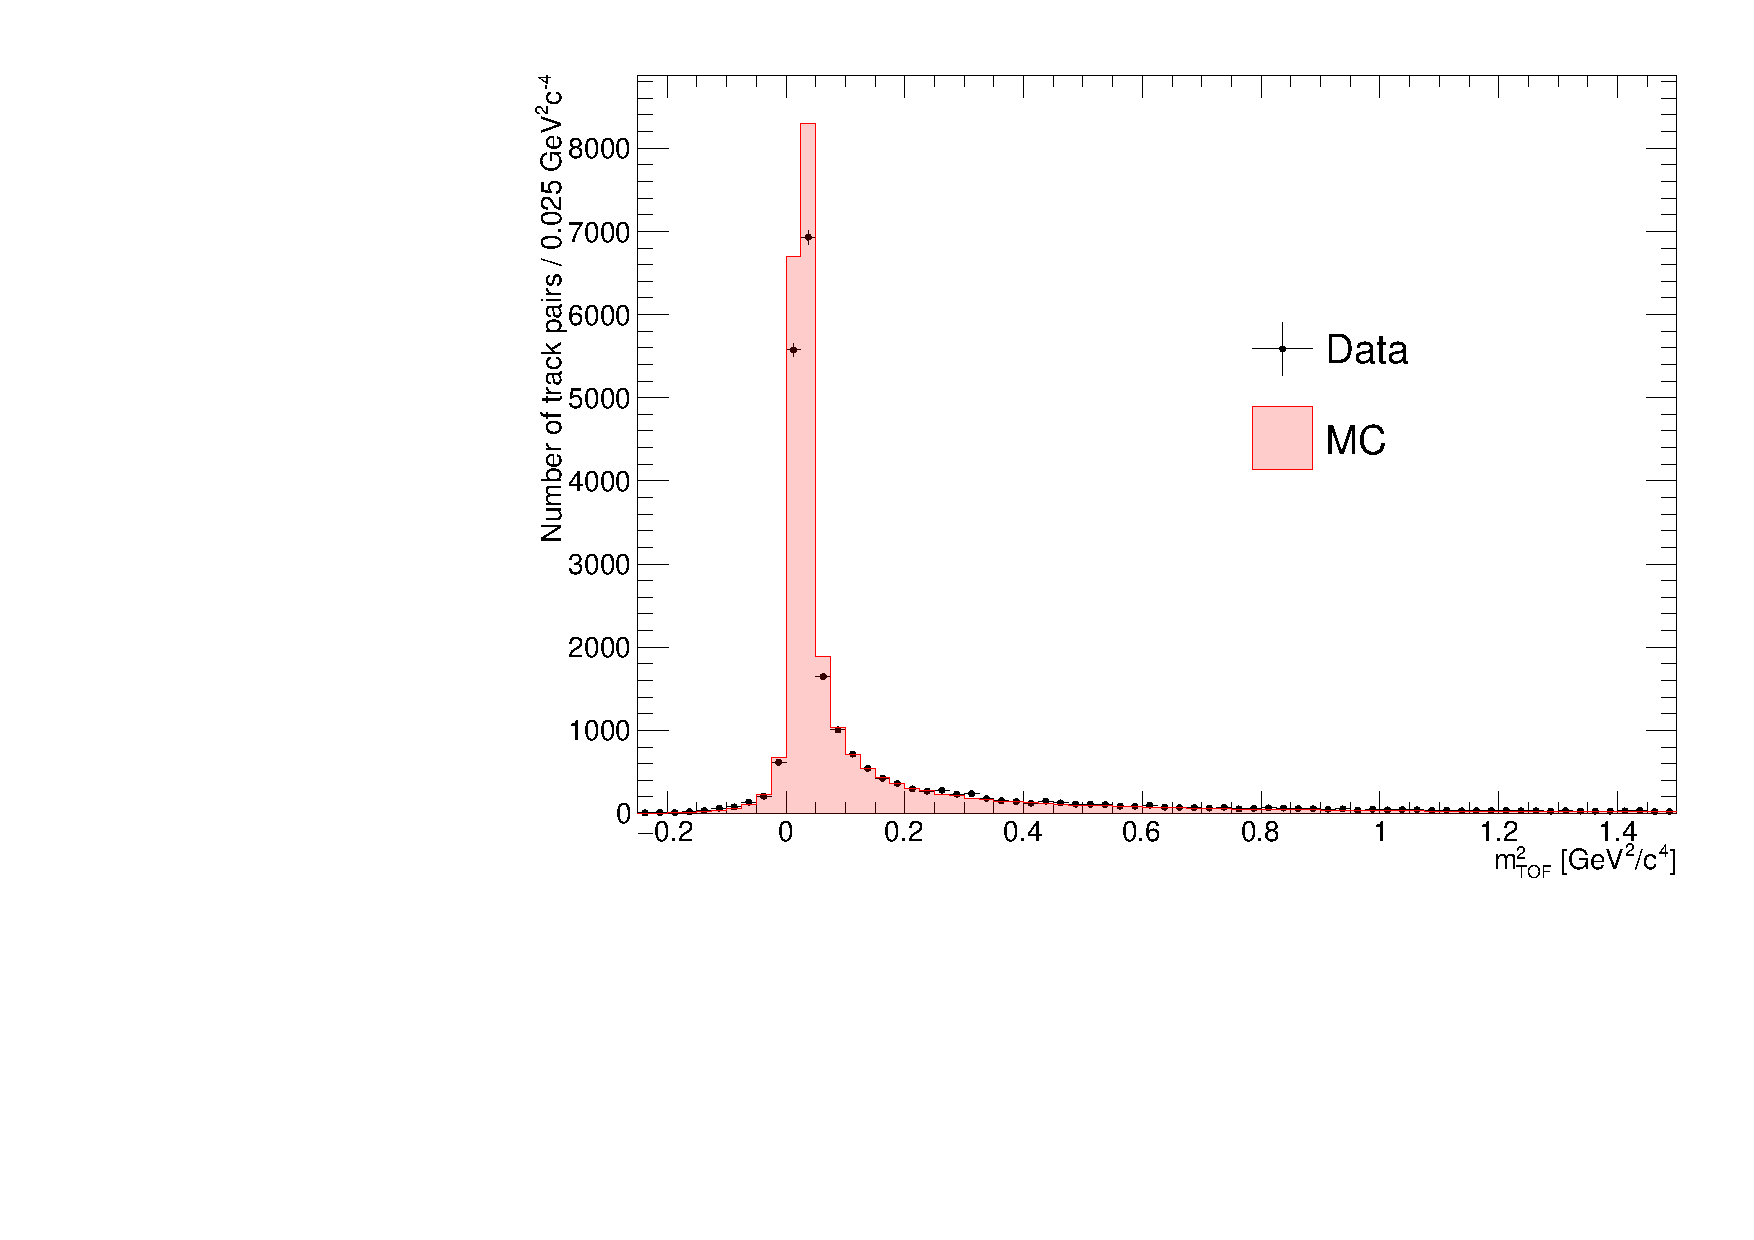
\includegraphics[width=\linewidth,page=1]{graphics/corrections/sqMassTof_DataVsMC.pdf}}}
  \end{subfigure}
}
\quad
\parbox{0.315\textwidth}{
  \centering
  \begin{subfigure}[b]{\linewidth}{
                \subcaptionbox{\label{fig:sqMassTof_DataVsMC_kaon}}{\includegraphics[width=\linewidth,page=2]{graphics/corrections/sqMassTof_DataVsMC.pdf}}}
  \end{subfigure}
}
\quad
\parbox{0.315\textwidth}{
  \centering
  \begin{subfigure}[b]{\linewidth}{
                \subcaptionbox{\label{fig:sqMassTof_DataVsMC_proton}}{\includegraphics[width=\linewidth,page=3]{graphics/corrections/sqMassTof_DataVsMC.pdf}}}
  \end{subfigure}
}%
\caption{Comparison of $m^{2}$ from TOF between data and MC for exclusive $\pi^{+}\pi^{-}$, $K^{+}K^{-}$ and $p\bar{p}$.}
\end{figure}
%---------------------------









\subsection{RP track acceptance and reconstruction efficiency}\label{sec:rpAccAndEff}

\subsection{TPC vertex reconstruction efficiency}\label{sec:tpcVxRecoEff}

The definition of vertex reconstruction efficiency established in this analysis is the probability that two global tracks, both associated with true-level primary particles from the kinematic region of the measurement, both satisfying kinematic and quality criteria (cuts~\ref{enum:TpcKinematicCuts} and ~\ref{enum:TpcQualityCuts}) and both matched with hits in TOF, form a vertex listed in the collection of reconstructed primary vertices and DCA(R) and DCA(z) of both global tracks calculated w.r.t. this vertex is contained within the limits of cut~\ref{enum:TpcDcaCuts}.

\section{Particle energy loss}\label{sec:energyLoss}
\section{Background subtraction}\label{sec:bkgdSubtraction}
\section{Unfolding}\label{sec:unfolding}

% 
%   W analizie CEP wydajność werteksowania to prawdopodobieństwo że
%  oba pierwotne ślady z punktu B tworzą werteks (to znaczy są na liście
%  śladów primary wspólnego werteksu i spełniaja ciecia DCA).
%  Nie patrzymy na dodatkowe werteksy, hity w TOF, BBC_small
% 
% E) --- pozostałe wydajności
% 
%   w przypadku analizy CEP jest to pile-up czyli dodatkowy werteks lub
%   dodatkowy hit w TOF lub sygnał w BBC. Te poprawk mamy z embeddingu
%   patrząc ile przypadków z D ma dodatkowy werteks, hist w TOF lub BBC
% 
%   To samo powinniśmy dostać z analizy "naszych" zero-bias.
% 
%   W przypadku analizy SD mamy pile-up czyli dodatkowy werteks, BBC
%   po stronie protonu też to znamy z embeddingu lub "naszych" zero-bias.
% 
%   Dodatkowo dochodzą dodatkowe werteksy z oddziaływań wtórnych/rozpadów.
%   Ten efekt znamy z MC. Powinno być to samo z pile-up'em jak i  bez
% 
% 
% Jakieś uwagi?
